\documentclass[a4paper, 18pt]{article}
\usepackage[T1]{fontenc}
\usepackage[utf8]{inputenc}
\usepackage[portuguese]{babel}
\usepackage[margin=3cm,includefoot,footskip=30pt]{geometry}

\usepackage{graphicx}
\graphicspath{ {imagens/} {flowcharts/}}
\usepackage{bold-extra}
\usepackage{epstopdf}
\usepackage{float}
\usepackage{scalerel}
\usepackage{enumerate}
\usepackage{indentfirst}
\usepackage{mathtools}
\usepackage{amsmath}
\allowdisplaybreaks
\usepackage{cleveref}
\usepackage{amssymb}
\usepackage{listings}
\usepackage{color}
\usepackage{textcomp}
\newcommand\showdiv[1]{\overline{\smash{\hstretch{.5}{)}\mkern-3.2mu\hstretch{.5}{)}}#1}}
\newcommand\ph[1]{\textcolor{white}{#1}}
\newcommand\tu[1]{\textunderscore}


\definecolor{dkgreen}{rgb}{0,0.6,0}
\definecolor{gray}{rgb}{0.5,0.5,0.5}
\definecolor{mauve}{rgb}{0.58,0,0.82}
\definecolor{mygreen}{RGB}{28,172,0} % color values Red, Green, Blue
\definecolor{mylilas}{RGB}{170,55,241}

% ----- Cabeçalho e rodapé -----
\usepackage{fancyhdr}
\pagestyle{fancy}
\fancyhf{}

\renewcommand{\headrulewidth}{1pt}
\renewcommand{\footrulewidth}{0.5pt}

\rhead{Word Morph}
\lhead{Algoritmos e Estruturas de Dados\rightmark}
\rfoot{Página \thepage}
\lfoot{\small Engenharia Eletrotécnica e de Computadores - IST}


\usepackage{pdfpages}

\begin{document}

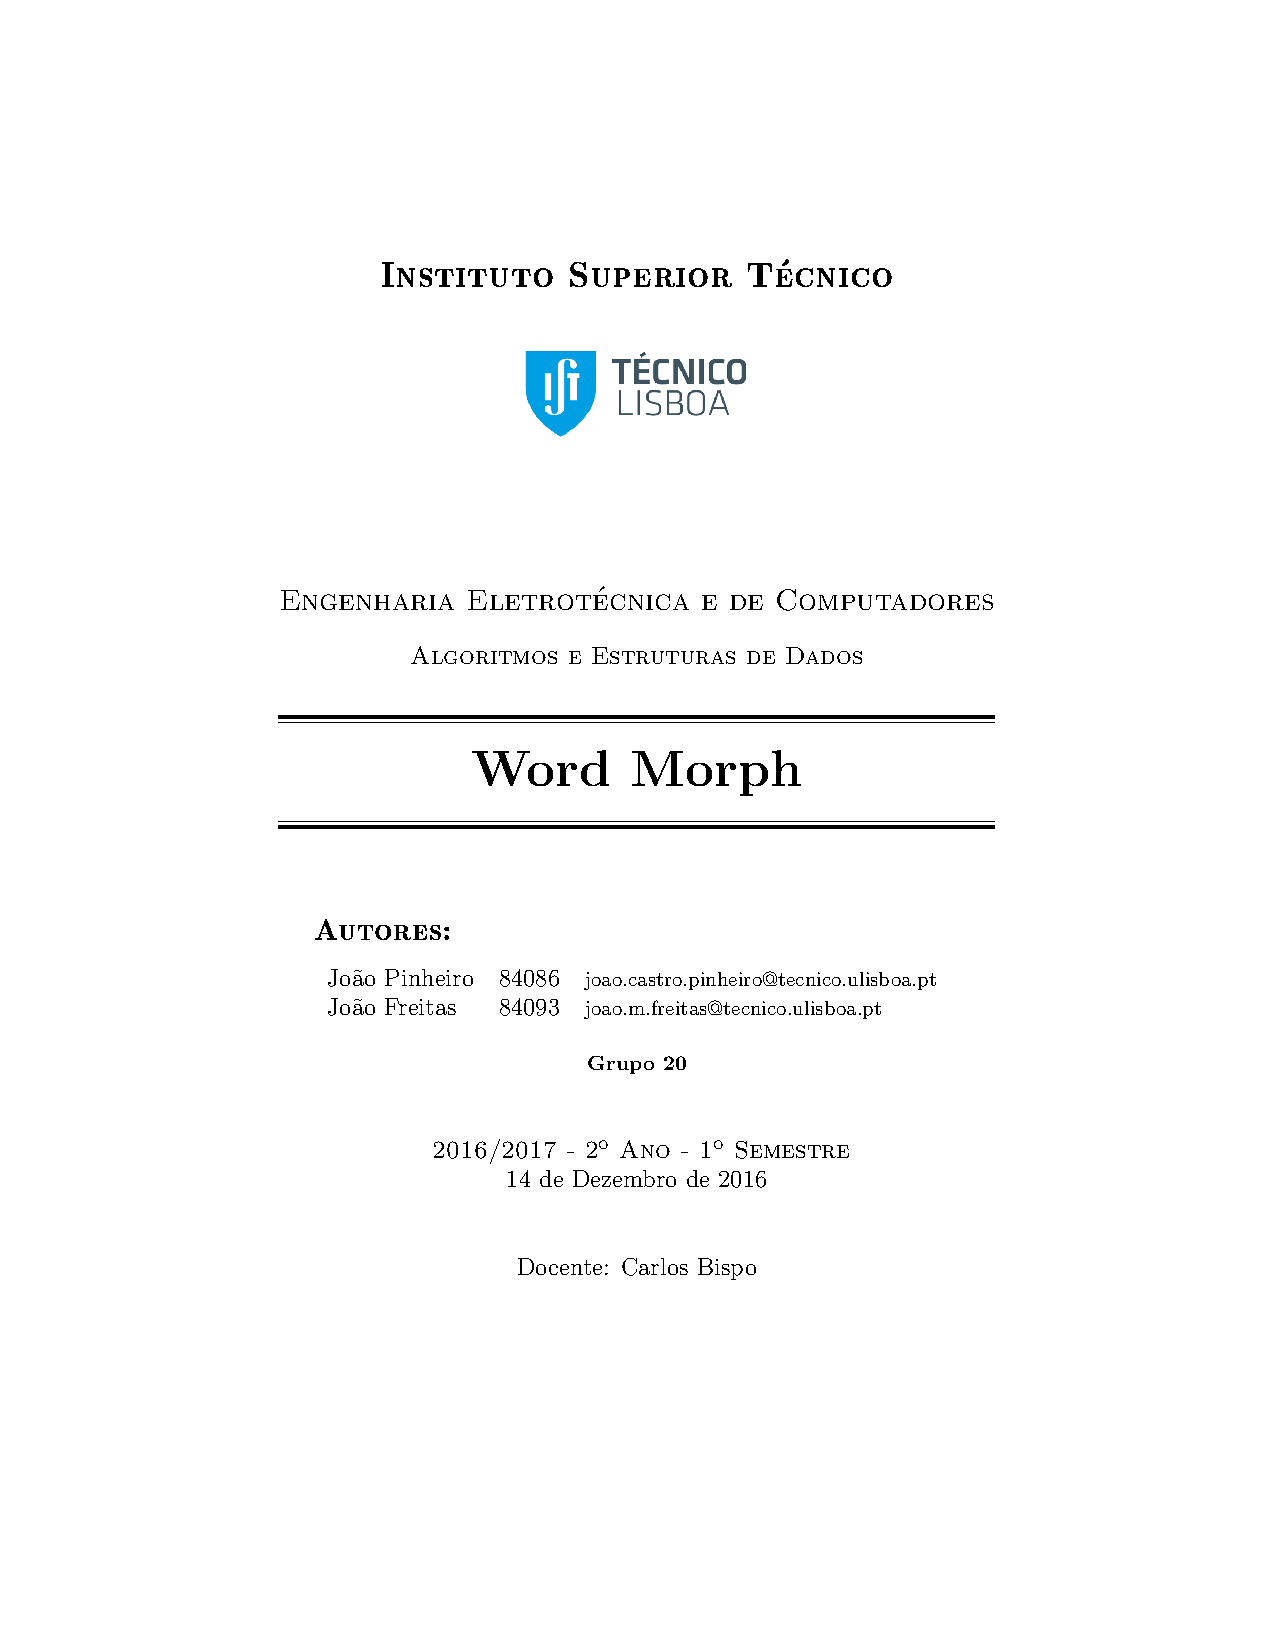
\includepdf[pages={1}]{capa/capa.pdf}

\tableofcontents
\newpage

\section{Especificação do problema}
	\par
	O problema proposto é encontrar caminhos entre duas palavras do mesmo tamanho. Estes caminhos consistem em permutações de letras. Em cada passo podem-se alterar no máximo um dado número de letras. No entanto, o peso duma ligação é o quadrado do número de carateres mudados. O objetivo é então encontrar o caminho de menor custo (i.e., que minimiza o peso total das ligações do caminho) entre a palavra de origem e a palavra de destino, passando por palavras do dicionário dado. Por exemplo, dado o problema:
	\begin{center}
		\texttt{dragar oravam 2}
	\end{center}
	\par
	É preciso encontrar o caminho de \textbf{dragar} a \textbf{oravam}, permutando, no máximo, 2 palavras em cada passo. Um caminho válido é então:
	\begin{center}
		\textbf{dragar} \\
		tragam \\
		\textbf{oravam}
	\end{center}
	\par
	Através de duas mutações de dois carateres cada. O custo total deste caminho é $2 \times 2^2 = 8$. No entanto, um caminho de menor custo seria:
	\begin{center}
		\textbf{dragar} \\
		tragar \\
		tragam \\
		travam \\
		\textbf{oravam}
	\end{center}
	\par
	Através de 4 mutações de um carater cada. O custo total deste caminho é $4 \times 1^1 = 4$, sendo de menor custo do que o anterior e, deste modo, a resposta correta.
	\par
	Para resolver grandes quantidades destes problemas, implementou-se uma solução na linguagem \textit{C}.
	O programa recebe dois parâmetros: \\
	\begin{itemize}
		\item Um ficheiro de dicionário de extensão \texttt{.dic} de palavras não acentuadas, não hifenadas e não necessariamente ordenado alfabeticamente, no formato de palavras separadas por um só espaço e uma ou mais palavras por linha.
		\item Um ficheiro de problemas de extensão \texttt{.pal} com vários problemas, um por linha, no formato:
		\begin{center}
		\texttt{<origem> <destino> <número máximo de permutações>}
		\end{center}
		\par
		Onde se assume que o formato está correto e as palavras pertencem ao dicionário.
	\end{itemize}
	\par
	O programa é invocado então da seguinte maneira:
	\begin{center}
		\texttt{\$ ./wordmorph <dicionário.dic> <problemas.pal>}
	\end{center}
	\par
	O programa escreve um ficheiro de saída de extensão \texttt{.path}, explicitando os caminhos e o custo associado, no seguinte formato, por exemplo, para o exemplo anterior \texttt{dragar oravam 2}:
	\begin{center}
		\texttt{
		dragar 4\\
		tragar \\
		tragam \\
		travam \\
		oravam}
	\end{center}
	\par
	É de notar que se não existir caminho, o peso será \texttt{-1}; se as palavras forem iguais, o peso será \texttt{0}. Existe uma linha em branco entre cada solução.


\section{Abordagem ao problema}
	\par
	Este problema é muito facilmente transposto num problema de grafos ponderados, em que os vértices representam palavras e as arestas ligações de $k$ permutações, sendo o peso da aresta igual a $k^2$. Calcular os caminhos mais curtos entre palavras traduz-se então num problema de caminho mais curto em grafos, onde se conhecem algoritmos de boa complexidade tanto temporal como de memória.


\section{Arquitetura}
	\par
	Os seguintes fluxogramas ilustram a arquitetura do programa no geral, incluindo referências às principais funções utilizadas:
	%\begin{figure}[H]
	%	\centering
	%	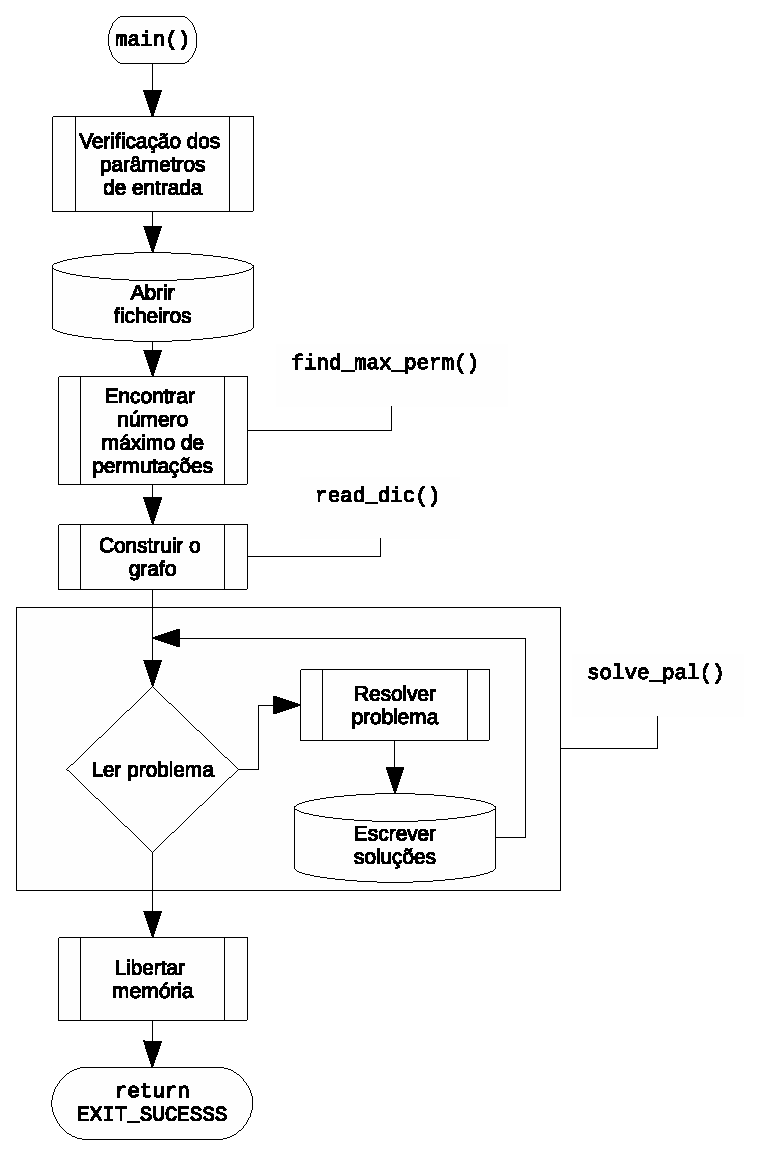
\includegraphics[width=0.6\linewidth]{main.eps}
	%	\caption{Fluxograma principal do programa (função \texttt{main}).}
	%\end{figure}
	%\begin{figure}[H]
	%	\centering
	%	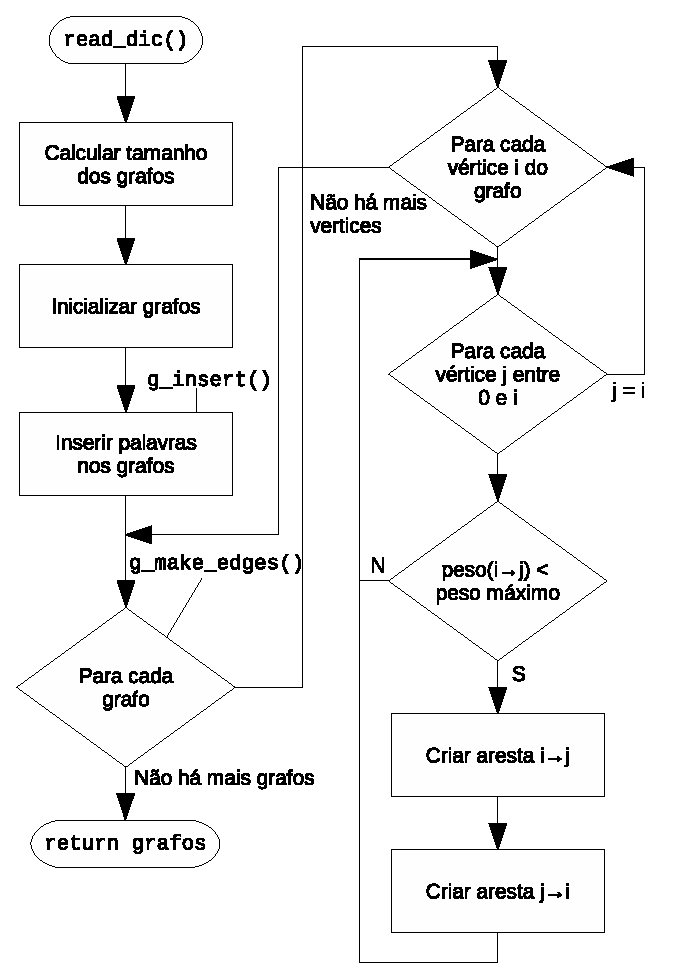
\includegraphics[width=0.85\linewidth]{read_dic.eps}
	%	\caption{Fluxograma da função \texttt{read\tu dic} que constrói o grafo.}
	%\end{figure}

	\par
	As estruturas de dados, algoritmos e subsistemas utilizados no programa serão descritos mais aprofundadamente nas próximas secções.
	\par
	Uma descrição completa da arquitectura do programa, incluindo fluxogramas
detalhados e um texto claro, mas sucinto, indicando a divisão lógica e funcional dos
módulos desenvolvidos para a resolução do problema, explicitando os respectivos
objectivos, as funções utilizadas e as estruturas de dados de suporte;


\section{Estruturas de dados}
	\par
	Como podem existir vários tamanhos de palavras no ficheiro de problemas, decidiu-se utilizar uma tabela de grafos indexada por um inteiro representando o tamanho de palavras que um grafo contém. Para construir os vários grafos, lê-se o ficheiro de problemas para perceber quais tamanhos de palavras e o respetivo número máximo de permutações serão necessários. De seguida, criam-se as arestas no grafo de acordo com este número, comparando palavra a palavra. Para resolver os problemas, utiliza-se um algoritmo de caminho mais curto no grafo pertinente.
	\begin{itemize}
		\item array de graph
		\begin{itemize}
			\item array de vertex
			\begin{itemize}
				\item lista (implícita) de edge
			\end{itemize}
		\end{itemize}

		\item heap
	\end{itemize}
	\par
	Uma descrição detalhada dos tipos de dados utilizadas e justificação dos mesmos
(tabelas, listas, filas, pilhas, árvores, grafos, acervos, etc.);

\section{Algoritmos}
			Para o cálculo de caminhos mais curtos entre palavras foi utilizado
			o algoritmo de Dijkstra.
			\begin{figure}[H]
				\centering
				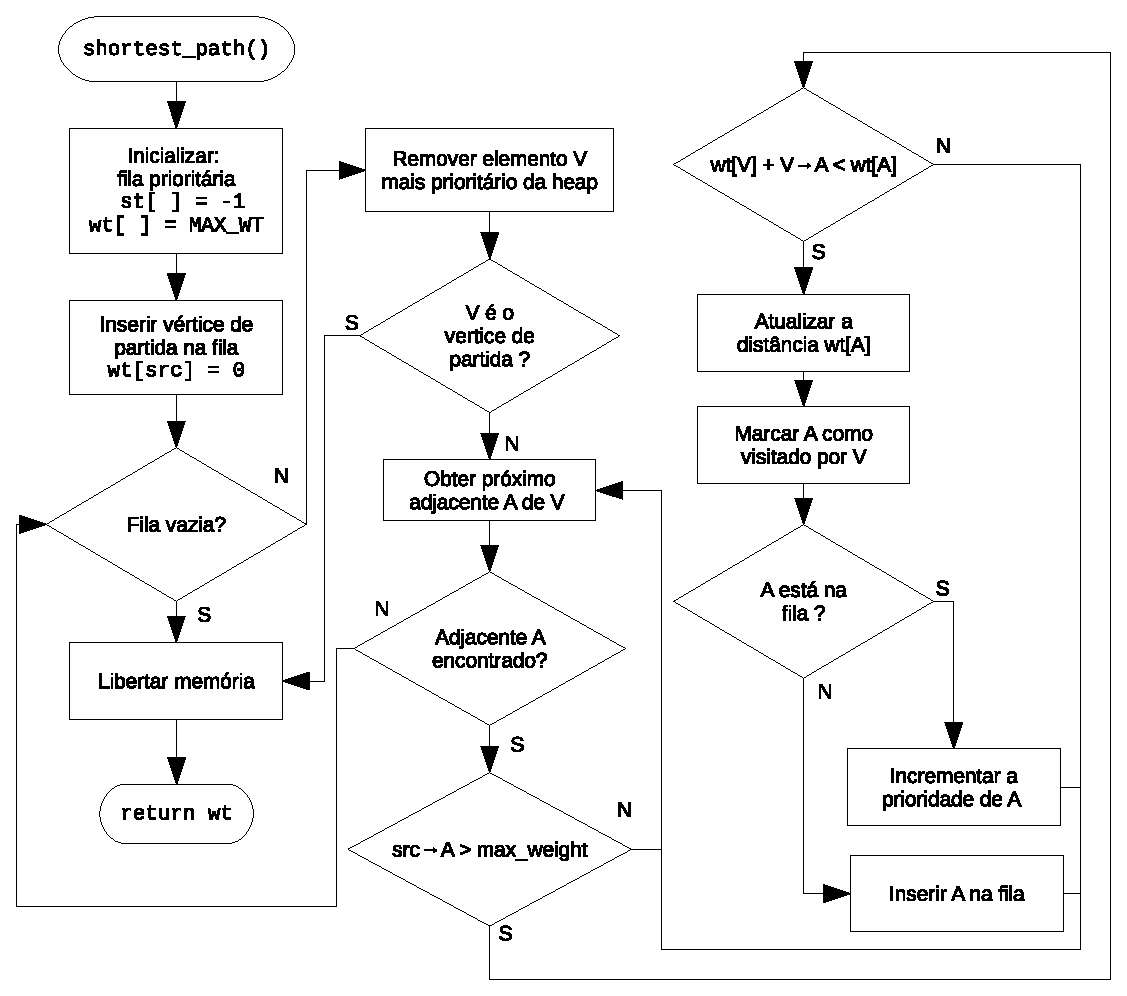
\includegraphics[width=\linewidth]{dijkstra}
				\caption{Algoritmo de Dijkstra}
			\end{figure}

	\begin{itemize}
		\item dijkstra
		\item heap: fixup, fixdown, insert, incpri, delmaxpri
		\item g\tu make\tu edges, g\tu insert, g\tu get\tu vertex
		\item fprint\tu path
	\end{itemize}
	\par
	Descrição dos algoritmos usados (por exemplo, na manipulação dos tipos de dados);

\section{Subsistemas}
	\begin{itemize}
		\item file.c
		\item heap.c
		\item graph.c
		\item dijkstra.c
		\item word.c
	\end{itemize}
	\par
	Uma descrição dos subsistemas funcionais que existam e, para cada um:
	– a descrição dos objectivos do subsistema (até 5 linhas);
	– o nome do módulo onde estão definidos os tipos de dados abstractos
	  (ficheiros .h) a utilizar no subsistema;
	– o nome do módulo C onde estão as funções do respectivo subsistema;
	– listagem das funções implementadas no subsistema, indicando para cada uma a
	  respectiva assinatura e os objectivos da função (descrição sumária, sem código);

\section{Análise de complexidade}
	\par
	Tempo
	\begin{itemize}
		\item fors do file.c $\Theta(n)$
		\item dijkstra $\Theta((E+V) lg V)$
		\item g\tu make\tu edges $\Theta(\frac{1}{2}V^2) = \Theta(V^2)$
	\end{itemize}
	\par
	Memória
	\begin{itemize}
		\item memoria: $\Theta(V + E)$
	\end{itemize}
	\par
	Uma análise, formal e/ou empírica, dos requisitos computacionais do programa desenvolvido, tanto em termos da memória que utiliza como da complexidade computacional, com particular ênfase no custo das operações de processamento sobre os tipos de dados usados e/ou criados;

\section{Análise crítica}
	\par
	Ideia: falar de como utilizarmos listas abstratas ao início, mas percebemos que estas gastavam demasiada memória e por isso tivemos de utilizar uma solução com listas ''implícitas'' na estrutura \texttt{Vertex}.
	\par
	Uma análise crítica do funcionamento do programa e a avaliação do desempenho
do projecto implementado;

\section{Exemplo de execução}
	\par
	Por exemplo, para o ficheiro de problemas:
	\begin{center}
		\texttt{tragar travam 2}
	\end{center}
	\par
	E para o dicionário:
	\begin{center}
		\texttt{tragar tragam travam a flores}
	\end{center}
	\par
	Depois de verificar os parâmetros de entrada e abrir os ficheiros, \texttt{find\tu max\tu perms()} é chamada.
	Inicializa \texttt{max\tu perms} a zero e de seguida o ficheiro de problemas é lido: como \texttt{w\tu diff()} devolve 2 e \texttt{max\tu perms[6] = 0 < 2}, então \texttt{max\tu perms[6] = 2} e os valores nos restantes índices ficam iguais a zero.
	\par
	A seguir constrói-se o grafo, chamando \texttt{read\tu dic()}. Esta função primeiramente lê o dicionário à procura do número de palavras de cada tamanho a alocar e chega apenas a \texttt{num\tu words[6] = 4}, ignorando a palavra de tamanho 1  pois \texttt{max\tu perms[1] = 0}. Seguidamente, \texttt{graphs[6]} é inicializado com 4 vértices (palavras), ficando os restantes valores nos índices \texttt{i} de \texttt{graphs} iguais a \texttt{NULL} pois representam os restantes tamanhos de palavra em que \texttt{max\tu perms = 0}. Agora o dicionário é lido outra vez para alocar as palavras em si, sendo \texttt{g\tu insert()} e \texttt{w\tu new()} chamadas 4 vezes, correspondendo às 4 palavras de tamanho 6. A seguir é chamada \texttt{g\tu make\tu edges()} para construir as arestas entre os vértices do grafo de tamanho de palavra 6. A tabela de vértices é:
	\texttt{[0: "tragar", 1: "tragam", 2: "travam", 3: "flores"]}
	\par
	Os resultados dos ciclos em \texttt{g\tu make\tu edges()} são apresentados de seguida:
	\begin{itemize}
		\item
			\texttt{i = 0, j = 0} \\
			\texttt{---------------------}
		\item
			\texttt{i = 1, j = 0} \\
			\texttt{calc\tu weight("tragam", "tragar", 2) = 1} \\
			\texttt{e\tu add(g, 1 ("tragam"), 0 ("tragar"), 1)}
		\item
			\texttt{i = 2, j = 0} \\
			\texttt{calc\tu weight("travam", "tragar", 2) = 2} \\
			\texttt{e\tu add(g, 2 ("travam"), 0 ("tragar"), 4)}
		\item
			\texttt{i = 2, j = 1} \\
			\texttt{calc\tu weight("travam", "tragam", 2) = 1} \\
			\texttt{e\tu add(g, 2 ("travam"), 1 ("tragam"), 1)}
		\item
			\texttt{i = 3, j = 0} \\
			\texttt{calc\tu weight("flores", "tragar", 2) = 3}
		\item
			\texttt{i = 3, j = 1} \\
			\texttt{calc\tu weight("flores", "tragam", 2) = 3}
		\item
			\texttt{i = 3, j = 2} \\
			\texttt{calc\tu weight("flores", "travam", 2) = 3}
	\end{itemize}
	\par
	O grafo resultante como representado no programa, sob listas de adjacências (à direita) e graficamente (à esquerda) é: \\
	\begin{minipage}{\linewidth}
		\centering
		\begin{minipage}{0.45\linewidth}
		\begin{center}
			\texttt{0: 1 \textrightarrow{} 2 \textrightarrow{} NULL \\
					1: 0 \textrightarrow{} 2 \textrightarrow{} NULL \\
					2: 0 \textrightarrow{} 1 \textrightarrow{} NULL \\
					3: NULL}
		\end{center}
		\end{minipage}
		\hspace{0.05\linewidth}
		\begin{minipage}{0.45\linewidth}
			\begin{figure}[H]
				\centering
				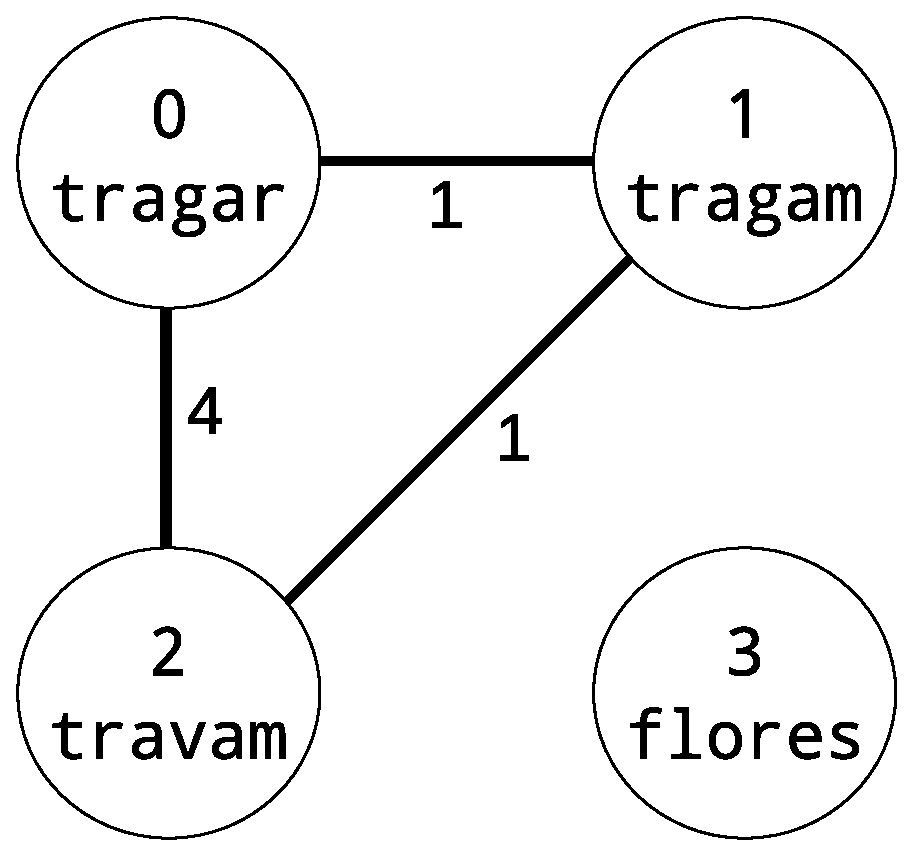
\includegraphics[width=4cm]{graph}
				\caption{Representação gráfica do grafo de exemplo}
			\end{figure}
		\end{minipage}
	\end{minipage} \\
	\par
	Construído o grafo, salta-se para a função \texttt{solve\tu pal()}. O ficheiro de problemas é lido outra vez. Como \texttt{w\tu diff("tragar", "travam", 1) = 2 > 1}, a solução não é trivial. Deste modo, encontramos o vértice de origem, correspondente a \texttt{"tragar"} e o de destino \texttt{"travam"}, (re)aloca-se a árvore de caminhos \texttt{path} e corre-se \texttt{shortest\tu path()}.
	\par
	Esta função primeiramente inicializa um acervo, (re)aloca a tabela de distâcias à origem \texttt{wt} e inicializa-a com o valor \texttt{MAX\tu WT} representando uma distância infinita e inicializa a árvore de caminhos \texttt{st} com \texttt{-1} sinalizando que nenhum vértice foi visitado. O vértice de origem é também inserido no acervo inicialmente e a sua distância à origem é colocada a \texttt{0}. Apresenta-se o estado final das sucessivas iterações do ciclo \texttt{while} exterior do algoritmo de Dijkstra:
	\begin{center}
		\begin{minipage}{0.45\linewidth}
		\texttt{\\
		v = 0\\
		v != dst (= 2) \\
		wt = [0, 1, 4, MAX\tu WT] \\
		st = [-1, 0, 0, -1] \\
		heap = [1, 2] \\}
		\end{minipage}
	\end{center}
	\par
	Na primeira iteração, o vértice \texttt{0} saiu da fila e foram colocados os seus adjacentes \texttt{1} e \texttt{2}, tendo sido marcados como visitados por \texttt{0} em \texttt{st} e com distâncias, respetivamente, \texttt{1} e \texttt{4} em \texttt{wt}. O acervo ficou com o vértice \texttt{1} na posição 0 mais prioritária então por este ter menor distância e assim maior prioridade. Assim, o vértice 1 sairá do acervo na próxima iteração:
	\begin{center}
		\begin{minipage}{0.45\linewidth}
			\texttt{\\
			v = 1\\
			v != dst (= 2) \\
			wt = [0, 1, 2, MAX\tu WT] \\
			st = [-1, 0, 1, -1] \\
			heap = [2] \\}
		\end{minipage}
		\hspace{0.05\linewidth}
	\end{center}
	\par
	Os vértices adjacentes de 1 são \texttt{0} e \texttt{2}, mas \texttt{0} não entrará no acevo pois a sua distância (\texttt{0}) já é menor do que vista pelo vértice \texttt{1} (\texttt{1}). O vértice \texttt{2} tem a sua prioridade incrementada, pois, a partir do vértice \texttt{1}, a sua distância à origem é \texttt{wt[1] + 1 = 1 + 1 = 2} que é menor que a previamente encontrada de \texttt{wt[2] = 4}. Assim, o vértice 2 passa a ocupar a posição mais prioritária no acervo e sairá deste na próxima iteração:
	\begin{center}
		\begin{minipage}{0.45\linewidth}
		\texttt{\\
			v = 2 \\
			v == dst \\
			wt = [0, 1, 2, MAX\tu WT] \\
			st = [-1, 0, 1, -1] \\
			heap = [2] \\}
		\end{minipage}
		\hspace{0.05\linewidth}
	\end{center}
	\par
	O vértice de destino saiu do acervo e parou-se a procura. A execução regressa a \texttt{solve\tu pal()} que escreverá o peso \texttt{wt[dst] = 2} e o caminho para este problema:
	\begin{center}
	\begin{minipage}{0.15\linewidth}
		\texttt{tragar 2 \\
				tragam \\
				travam}
	\end{minipage}
	\end{center}
	\par
	Onde o caminho foi impresso na ordem correta pela função recursiva \texttt{fprint\tu path()} (seguindo o caminho para trás desde \texttt{st[dst]} até chegar ao ponto inicial onde \texttt{st[src] = -1}):
\end{document}
